\documentclass[conference]{IEEEtran}
\IEEEoverridecommandlockouts
% The preceding line is only needed to identify funding in the first footnote. If that is unneeded, please comment it out.
\usepackage{cite}
\usepackage{amsmath,amssymb,amsfonts}
\usepackage{algorithmic}
\usepackage{graphicx}
\usepackage{textcomp}
\usepackage{xcolor}

% begin DWei added #1
\usepackage{fancyhdr}
\fancyhf{} % comment this to show page number on center footer
\pagestyle{fancy}
\rfoot{\parbox{3.5in}{\raggedleft\fontsize{8pt}{10pt} \selectfont \textcolor{gray}{The 9th Asia-Pacific International Symposium on Advanced Reliability and Maintenance Modeling  (APARM 2020 -- Vancouver)}}}
% end DWei added #1

\def\BibTeX{{\rm B\kern-.05em{\sc i\kern-.025em b}\kern-.08em
    T\kern-.1667em\lower.7ex\hbox{E}\kern-.125emX}}
\begin{document}

\title{A Predictive Maintenance framework Through the Event-based Genomics of Machine Breakdown*\\
\thanks{This project has received funding from the European Union's Horizon 2020 research and innovation program under grant agreement Nos 768869 (Z-BRE4K) and 723906 (Z-FACT0R).}
}

\author{\IEEEauthorblockN{Morad Danishvar}
\IEEEauthorblockA{\textit{College of Engineering, Design and} \\ \textit{Physical Sciences} \\
\textit{Brunel University}\\
London, UK \\
Morad.Danishvar@brunel.ac.uk}\\
\and
\IEEEauthorblockN{Veerendra C. Angadi}
\IEEEauthorblockA{\textit{College of Engineering, Design and} \\ \textit{Physical Sciences} \\
\textit{Brunel University}\\
London, UK \\
Veer.Angadi@brunel.ac.uk}\\
\and
\IEEEauthorblockN{Ali Mousavi}
\IEEEauthorblockA{\textit{College of Engineering, Design and} \\ \textit{Physical Sciences} \\
\textit{Brunel University}\\
London, UK \\
Ali.Mousavi@brunel.ac.uk}\\
}

\maketitle
% begin DWei added #2
\thispagestyle{fancy}
% begin DWei added #2

\begin{abstract}
This document is a model and instructions for \LaTeX.
This and the IEEEtran.cls file define the components of your paper [title, text, heads, etc.]. *CRITICAL: Do Not Use Symbols, Special Characters, Footnotes,
or Math in Paper Title or Abstract.
\end{abstract}

\begin{IEEEkeywords}
Real-time Event Sequencing, Genomics of Machine Breakdown, Predictive Maintenance, Regressive Event Tracker, remaining useful life, Machine Learning, Manufacturing, Data-driven, Compression Moulding Machine
\end{IEEEkeywords}


\section{Introduction}
\label{sec:Introduction}
This document is a model and instructions for \LaTeX.
Please observe the conference page limits.

\section{Related Works}
\label{sec:Related_works}


\section{Sequential Breakdown Prediction the Theory of Event-Base Genomics of Machine Breakdown (GMB)}
\label{sec:GMB}


\subsection{GMB Algorithm}
\label{subsec:GMB_Algorithm}

\begin{figure}[htbp]
\centerline{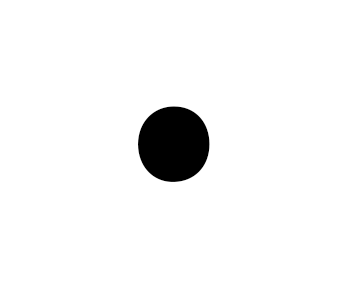
\includegraphics{fig1.png}}
\caption{Genome labelling and sequential differentiation example.}
\label{fig:Genome_labelling}
\end{figure}

\section{The DNA of continuous compression machine}
\label{sec:DNA_CCM}

\begin{figure}[htbp]
\centerline{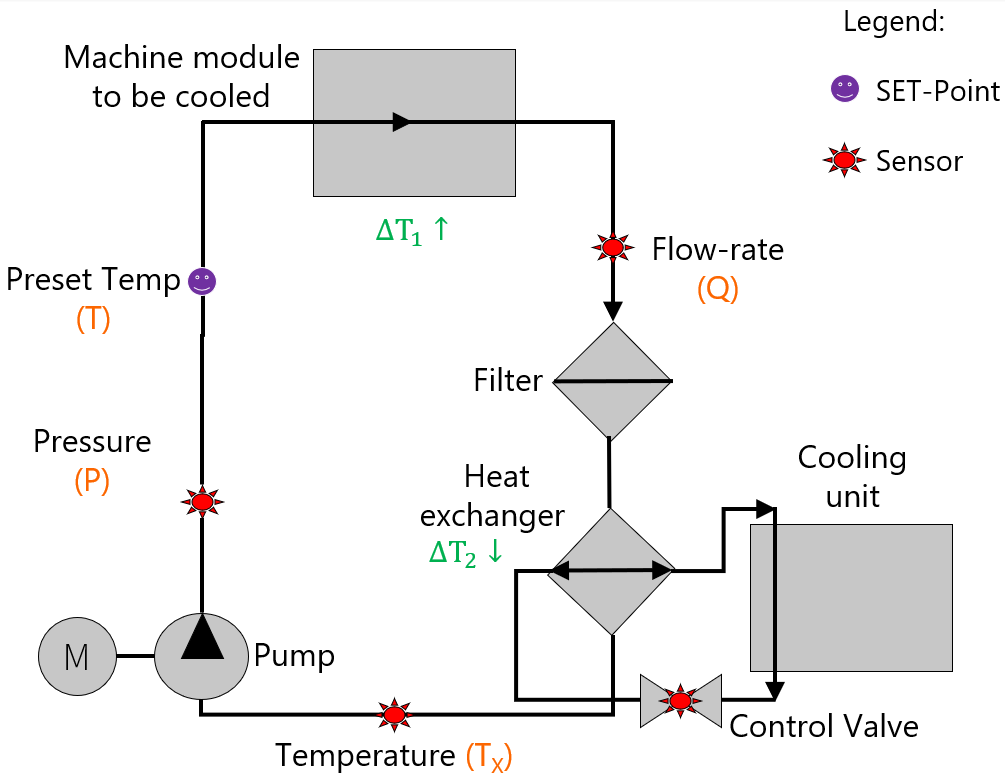
\includegraphics[width=0.45\textwidth]{TH_schematic.png}}
\caption{The flow diagram of the coolant in the thermal regulator.}
\label{fig:TH_schematic}
\end{figure}

\begin{figure}[htbp]
\centerline{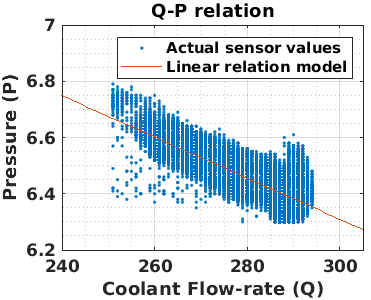
\includegraphics[width=0.45\textwidth]{QP_relation.png}}
\caption{The control system feedback relation between coolant flow-rate (Q) and the pressure (P).}
\label{fig:QP_relation}
\end{figure}

\begin{figure}[htbp]
\centerline{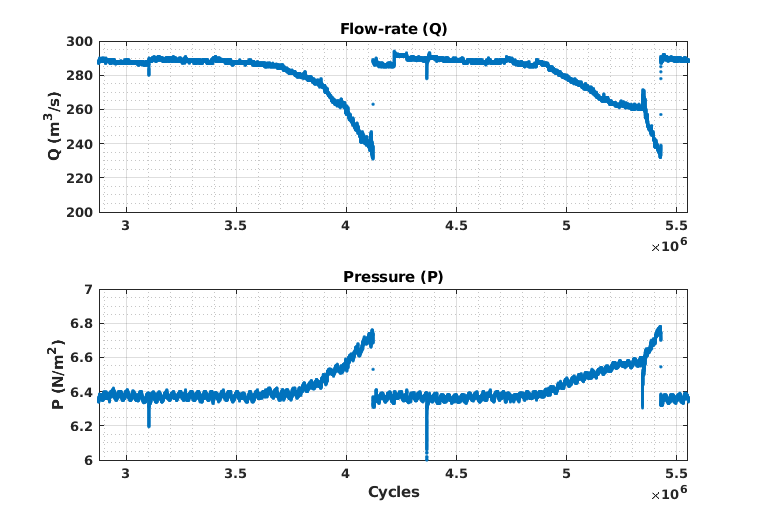
\includegraphics[width=0.45\textwidth]{Sensor_values.png}}
\caption{The coolant flow-rate and pressure sensor values after performing preventive maintenance by clearing the clogs in the filter.}
\label{fig:Sensor_values}
\end{figure}

\subsection{Event-Clustering sensitivity analysis algorithm}
\label{subsec:event_clustering}


\subsection{Safety threshold (ST)}
\label{subsec:ST}


\subsection{Genomes labelling and sequential differentiation }
\label{subsec:Genome_labelling}


\section{Regressive Event-Tracker}
\label{sec:RET}

\begin{figure}[htbp]
\centerline{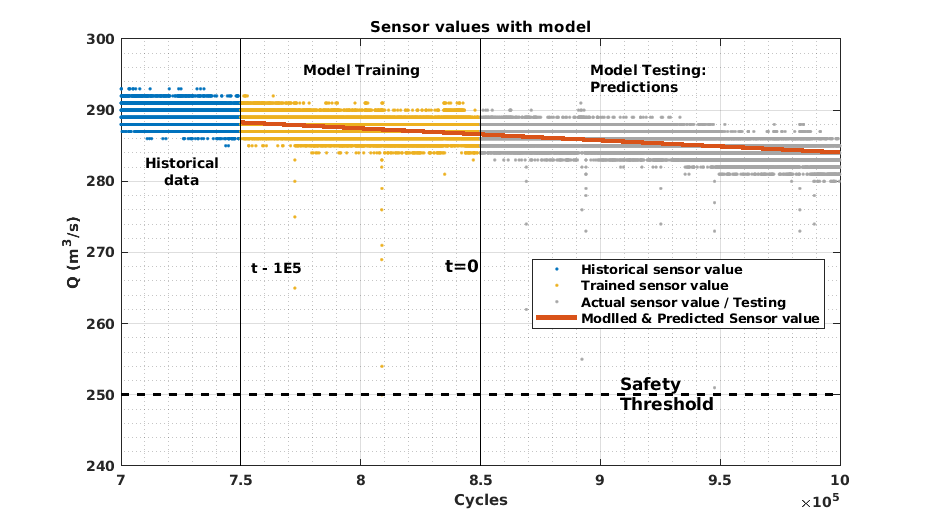
\includegraphics[width=0.45\textwidth]{Model.png}}
\caption{Sensor values of flow-rate training period of 105 cycles and prediction of sensor values and remaining useful life until the predicted values crosses the ST.}
\label{fig:Model}
\end{figure}

\subsection{Mean time to failure estimation for each sensors}
\label{subsec:MTTF}



\subsection{Estimation of lifetime of the thermal regulator}
\label{subsec:Lifetime}


\begin{table}[htbp]
\caption{Table Type Styles}
\begin{center}
\begin{tabular}{|c|c|c|c|}
\hline
\textbf{Table}&\multicolumn{3}{|c|}{\textbf{Table Column Head}} \\
\cline{2-4}
\textbf{Head} & \textbf{\textit{Table column subhead}}& \textbf{\textit{Subhead}}& \textbf{\textit{Subhead}} \\
\hline
copy& More table copy$^{\mathrm{a}}$& &  \\
\hline
\multicolumn{4}{l}{$^{\mathrm{a}}$Sample of a Table footnote.}
\end{tabular}
\label{tab1}
\end{center}
\end{table}

\begin{figure}[htbp]
\centerline{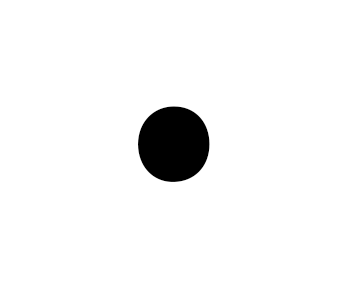
\includegraphics{fig1.png}}
\caption{Example of a figure caption.}
\label{fig}
\end{figure}

\section*{Acknowledgment}
\label{sec:Acknowledgment}
This project has received funding from the European Union's Horizon 2020 research and innovation program under grant agreement numbers 768869 (Z-BRE4K) and 723906 (Z-FACT0R).


\bibliographystyle{IEEEtran}
\bibliography{IEEEbib}

\end{document}
